\documentclass{article}
\usepackage{amsmath}
\usepackage{tikz}

\begin{document}
	
	To find the volume of a sphere using integration, we can use the method of slicing the sphere into small disks and summing up their volumes. In this explanation, we will consider a sphere with radius R and volume V.
	
	First, let's set up a coordinate system with the center of the sphere at the origin (0, 0, 0). We can express the radius r of a disk at a given height z as a function of z. To do this, we will use the Pythagorean theorem:
	
	\[r^2 + z^2 = R^2\]
	
	Solving for r as a function of z, we get:
	
	\[r(z) = \sqrt{R^2 - z^2}\]
	
	\begin{figure}[h]
		\centering
		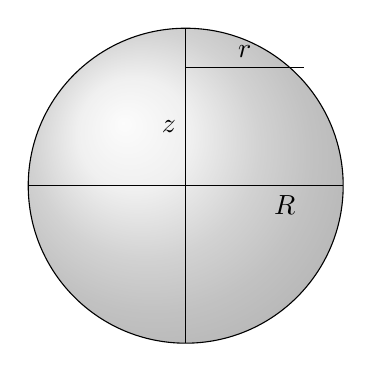
\begin{tikzpicture}
			\shade[ball color = gray!40, opacity = 0.4] (0,0) circle (2cm);
			\draw (0,0) circle (2cm);
			\draw (-2,0) -- (2,0);
			\draw (0,-2) -- (0,2);
			\draw[dashed] (0,0) -- (2,0);
			\node[below right] at (1,0) {$R$};
			\draw[dashed] (0,0) -- (0,1.5);
			\node[left] at (0,0.75) {$z$};
			\draw (0,1.5) -- (1.5,1.5);
			\node[above] at (0.75,1.5) {$r$};
		\end{tikzpicture}
		\caption{A sphere with radius R and a disk at height z with radius r.}
	\end{figure}
	
	
	Now, let's consider a small disk of thickness $dz$ at height $z$. The volume of this disk is given by:
	
	\[dV = \pi \cdot r(z)^2 \cdot dz\]
	
	Substitute the expression for $r(z)$:
	
	\[dV = \pi \cdot \left(\sqrt{R^2 - z^2}\right)^2 \cdot dz\]
	
	\[dV = \pi \cdot (R^2 - z^2) \cdot dz\]
	
	Now we integrate dV with respect to z from the bottom hemisphere (z = -R) to the top hemisphere (z = R):
	
	\[V = \int_{-R}^{R}(\pi \cdot (R^2 - z^2) \cdot dz)\]
	
	Solve the integral:
	
	\[V = \pi \int_{-R}^{R}(R^2 - z^2) \cdot dz\]
	
	\[V = \pi \left[R^2 \left[z\right]_{-R}^{R} - \left[\frac{z^3}{3}\right]_{-R}^{R}\right]\]
	
	\[V = \pi \left[R^2 (R - (-R)) - \left(\frac{R^3}{3} - \frac{-R^3}{3}\right)\right]\]
	
	\[V = \pi \left[\frac{4R^3}{3}\right]\]
	
	\[V = \pi \left[\frac{4R^3}{3}\right]\]
	
	
	\[V = \frac{4}{3} \cdot \pi \cdot R^3\]
	
	Thus, the volume of a sphere with radius R is $\frac{4}{3}\pi R^3$, which is the familiar formula.
	
\end{document}